%
\chapter{Noções Elementares de Cálculo}
\section{Preliminares}
%%%%
Antes de estudar as sequências e séries de funções, recordamos alguns dos fatos básicos concernentes às funções contínuas e diferenciáveis, aos quais fizemos 
referências. Não apresentaremos demonstrações, embora tais demonstrações possam facilmente se basear nas, propriedades mais profundas do sistema de números reais 
tratadas em disciplinas de análise. Para um estudo completo, o leitor poderá se reportar a qualquer texto de Cálculo Avançado (ver, Marsden~\cite{mars}).

%%%%%
\section{Propriedades das Funções Elementares}
%%%%%%
\begin{defic}{Continuidade Pontual}{1115-6}
Dizemos que uma função $f$, definida num intervalo $I$ do eixo dos $x$, é \texttt{contínua} num ponto $x_{0}$ de $I$ se para todo $\vep > 0$ existe um $\de > 0$, dependente em geral 
de $\vep$ e $x_{0}$, tal que
\begin{equation*}
|f(x)-f(x_{0})| <\vep \quad \text{ para todos os pontos } \quad x \in I,
\end{equation*}
para os quais
\begin{equation*}
\|x-x_{0}\| <\de.
\end{equation*}
Se a função $f$ é contínua em todo ponto de $I$, dizemos que $f$ é contínua em $I$.
\end{defic}


Este é o conceito clássico de continuidade, fundamental para qualquer curso de cálculo elementar. Entretanto, não é geralmente introduzido nesse nível a seguinte noção de continuidade uniforme.

O conceito de continuidade de uma função num ponto é essencialmente de natureza local, o mesmo não se pode afirmar sobre a continuidade uniforme. A noção de continuidade uniforme de uma função é de caráter global porque afirmamos continuidade uniforme de uma função sobre seu domínio e não num ponto de seu domínio.

\begin{defic}{Continuidade Uniforme num Intervalo}{1115-7}
Uma função $f$ diz-se \texttt{uniformemente contínua} num intervalo $I$ se para todo $\vep > 0$ existe um $\de > 0$, dependente, em geral, de $\vep$  mas não de $x$, e tal que
\begin{equation*}
|f(x_1)-f(x_2)| < \vep \quad \text{ quando } \quad x_1, \;  x_2 \in I
\end{equation*}
e para os quais
\begin{equation*}
|x_1- x_2| < \de.
\end{equation*}
\end{defic}

É claro que uma função \texttt{uniformemente contínua} num intervalo é também \texttt{contínua} nesse intervalo. Porém, o seguinte exemplo mostra que a recíproca é falsa.

\begin{exer}
Seja a função $f$ real definida pela regra de correspondência,
\begin{equation*}
f(x) = \frac{1}{x}, \qquad 0 < x \le 1.  
\end{equation*}

Mostre que a função $f$ não é uniformemente contínua.
\end{exer}

\solo Seja $x_{_{0}}$ um ponto qualquer do intervalo $]0, \;1]$, isto é, fixamos $x_{_{0}}>0$. Para decidir como escolher $\delta$ devemos examinar a expressão
\begin{equation*}
  \left|\frac{1}{x}-\frac{1}{x_{0}}\right|=\frac{|x-x_{0}|}{|xx_{0}|}.
\end{equation*}

Se $|x-x_{_{0}}|<\de$, então teremos
\begin{equation*}
  \left|\frac{1}{x}-\frac{1}{x_{_{0}}}\right|=\frac{\de}{|xx_{_{0}}|}=\frac{\de}{xx_{_{0}}}.
\end{equation*}

Se verificarmos $\de<x_{_{0}}/2$, então deveríamos ter, $x-x_{_{0}}>x_{_{0}}/2$, portanto $x >x_{_{0}}/2$, de maneira  a ter que
\begin{equation*}
\frac{\de}{xx_{_{0}}}<\frac{2\de}{x_{_{0}}^2}.
\end{equation*}

Agora para cada $\varepsilon>0$, escolhemos
\begin{equation*}
  \delta=\min\left[\frac{x_{_{0}}}{2}, \;\frac{x_{_{0}}^2}{2}\vep \right]
\end{equation*}

Pelos argumentos anteriores mostramos que
\begin{equation*}
  \left|\frac{1}{x}-\frac{1}{x_{_{0}}}\right|<\vep\quad \text{sempre que }
  \quad |x-x_{_{0}}|<\de.
\end{equation*}

Assim temos satisfeitas as condições da Definição~\ref{def:1115-6}, e $f(x) = 1/x$ é contínua
em $x_{0}$, em decorrência no intervalo $0 < x \le 1$. Porém, o valor dado de $\de$ 
depende de $\vep$ e de $x_o$, e examinando a Figura~\ref{fig-111-3},
\begin{figure}[H]
\centering
\includegraphics[width=0.5\textwidth]{fig-111-3.eps}
\caption{Continuidade Uniforme}
\label{fig-111-3}
\end{figure}
convencemo-nos de que este é, necessariamente o caso.

Porque, dado qualquer $\vep > 0$ pode-se fazer com que os pontos $x'$, $x''$ da figura 
fiquem tão próximos de $x_{0}$ quanto se deseje, simplesmente escolhendo-se 
$x_{0}$ suficientemente próximo de $0$. Como se deve escolher $\de$ não maior do 
que $|x_{_{0}}- x'|$, tal fato mostra que ele não pode depender apenas de $\vep$. 
Portanto, $f$ \textit{não é uniformemente contínua} em $0 < x \le 1$. \hfill \(\lozenge\)

\bigskip
 A dificuldade neste exemplo provém, de que o intervalo $0 < x \le 1$ em consideração 
 não é um conjunto fechado. Isto é uma consequência do seguinte teorema geral.

\begin{theoc}{}{1115-13}
Se $f$ é uma função contínua num intervalo fechado $a \le x \le b$, então ela é 
uniformemente contínua neste intervalo.
\end{theoc}

Todos os conceitos expostos acima se estendem facilmente a funções de várias 
variáveis. Antes de iniciar, os enunciamos a seguir para fins de referência.

\begin{defic}{Continuidade de uma função escalar}{1115-8}
Uma função de valor real $f$ definida numa região $\Om$ de $\mathbb{R}^n$ é contínua 
no ponto $\mathbf{y} = (y_1,\ldots, y_n)$ de $\Om$ se para todo $\vep> 0$ existe 
um $\de> 0$, dependente, em geral, de $\vep$ e de
$\mathbf{y}$, tal que
\begin{equation*}
  |f(\mathbf{x}) - f(\mathbf{y})| = |f(x_1,\ldots, x_n)-f(y_1,\ldots, y_n) | < \vep
\end{equation*}
quando $\mathbf{x}$, $\mathbf{y}$ estão em $\Om$  e
\begin{equation*}
  \|\mathbf{y}-\mathbf{x}\|= \sqrt{(x_1-y_1)^2+\cdots+(x_n-y_n)^2} <\de.
\end{equation*}

Dizemos que $f$ é contínua em $\Om$ se ela é contínua em todo ponto de $\Om$.
\end{defic}

\begin{defic}{Continuidade Uniforme}{1115-9} 
Uma função $f$ é uniformemente contínua em $\Om$  se para 
todo $\vep >0$ existe um $\de > 0$, dependente, em geral, de $\vep$ mas não 
de $\mathbf{x}$, tal que
\begin{equation*}
  |f(\mathbf{x})-f(\mathbf{y}) |< \vep \quad \text{ quando } 
  \quad \mathbf{x}, \; \mathbf{y} \in \Om
\end{equation*}
sempre que
\begin{equation*}
  \|\mathbf{x}-\mathbf{y}\|<\de.
\end{equation*}
\end{defic}

Se considerarmos funções definidas em regiões $\Om$ limitadas e fechadas, teremos o 
seguinte teorema.
\begin{obs}
Uma região $\Om$ de $\mathbb{R}^n$ é fechada se ela contém todos os seus pontos 
limites. É limitada, se existe um número real $M$ tal que, para todo
 ponto $\mathbf{x} = (x_1,\ldots,  x_n)$ de $\Om$, temos
\begin{equation*}
\|\mathbf{x}\|=\sqrt{x_1^2+\cdots+x_n^2} \leq M.
\end{equation*}
\end{obs}

\begin{theoc}{}{1115-14} 
Se a função $f$ é contínua numa região $\Om$ limitada e fechada, então é uniformemente
contínua em $\Om$.
\end{theoc}

Duas propriedades das funções contínuas, são dadas pelos dois seguintes teoremas.

\begin{theoc}{Propriedade do Máximo e do Mínimo}{1115-15}
Se $f$ é contínua num intervalo fechado $a \le x \le b$, então ela assume aí um, valor máximo e um valor mínimo. De modo mais geral, se $f$ é contínua numa 
egião $\Om$ de $\mathbb{R}^n$ limitada e fechada, então existem números reais $m$, $M$ e pontos $\mathbf{y}=(y_1,\ldots y_n)$, $\mathbf{z} = (z_1,\ldots, z_n)$ em $\Om$, tais que
\begin{equation*}
  m \le f(\mathbf{x}) \le M
\end{equation*}
para todo $\mathbf{x} = (x_1,\ldots,x_n)$ em $\Om$, e tais que $f(\mathbf{y}) = m$ e $f(\mathbf{z})=M$.
\end{theoc}

\begin{theoc}{Propriedade do Valor Intermediário}{1115-16}
Se a função $f$ é contínua no intervalo $a \le x \le b$ e $f(a)\neq f(b)$, então para qualquer número 
real $M$ entre $f(a)$ e $f(b)$ existe um, ponto $x_o$, $a \le x_{_{0}} \le b$, tal 
que $f(x_{_{0}}) = M$. Enunciado análogo vale para funções de várias variáveis.
\end{theoc}

Embora estejamos familiarizados com os problemas de máximo e mínimo, pode passar despercebida a 
importância do Teorema~\ref{thm:1115-16}. Simplesmente, este teorema poderá, sem dúvida, ser 
utilizado para dar como certa a existência de raízes de equações; por exemplo, 
se $f(a) < 0$ e $f(b) > 0$ e se $f$ é contínua em $a \le x \le b$, então $f(x_{_{0}}) = 0$ 
para algum $x_{_{0}}$ deste intervalo. Mas a um nível mais profundo, o Teorema~\ref{thm:1115-16} 
é uma consequência das propriedades básicas do próprio sistema de números reais e pode ser 
interpretado como a de relacionar a noção intuitiva que temos de continuidade, com a definição
 abstrata de continuidade dada na Definição~\ref{def:1115-6}.

Passando agora às definições e teoremas relativos à derivação e à integração, enunciamos, primeiramente, a
\begin{defic}{Derivada de uma função real}{1115-10} 
Seja a função $f$ definida num intervalo aberto que contenha $x_{_{0}}$. Se existe
\begin{equation*}
  \lim_{h\to 0} \frac{f(x_o + h) - f(x_o)}{h}
\end{equation*}
chama-se ele derivada de $f$ em $x_{_{0}}$ e é representado por $f'(x_{_{0}})$ ou por $\dst{\frac{d}{dx}f(x_{_{0}})}$. Se $f$ tem derivada em cada ponto de um intervalo aberto $a < x < b$, então dizemos que $f$ é diferenciável neste intervalo.
\end{defic}

\begin{obs}
Mais adiante necessitaremos estender este conceito, para incluir também os extremos de um intervalo.
\end{obs}

Constitui simples exercício mostrar que, se $f$ \textit{é diferenciável num intervalo} $a < x < b$, \textit{então ela também é contínua neste intervalo}. Enunciemos, para referência, o teorema mais importante, em certo sentido.

\begin{theoc}{Teorema do Valor Médio}{1115-17} Se $f$ é contínua no intervalo 
fechado dado $a \le x \le b$ e diferenciável no intervalo aberto $a < x < b$, então 
existe um ponto $x_o$, $a < x_o < b$, tal que
\begin{equation*}
  \frac{f(b)-f(a)}{b-a}= f'(x_{0}).
\end{equation*}
\end{theoc}

A interpretação geométrica deste resultado acha-se ilustrada na Figura~\ref{fig-1115-4}.
\begin{figure}[H]
\centering
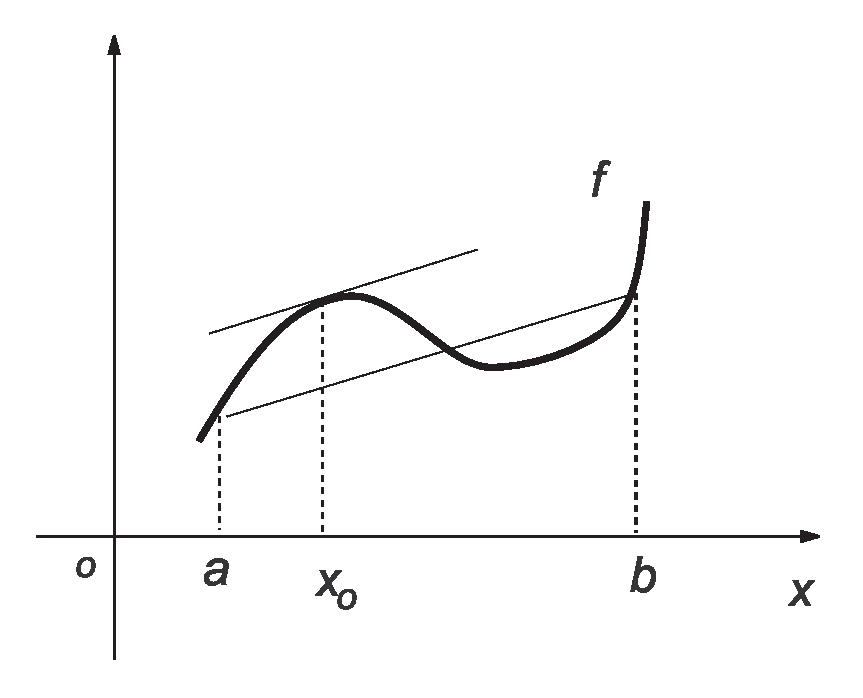
\includegraphics[width=0.45\textwidth]{fig-1115-4.eps}
\caption{Valor Médio} 
\label{fig-1115-4}
\end{figure}

Significa que existe pelo menos um ponto no intervalo aberto $a < x < b$, onde a tangente à curva $y = f(x)$ é paralela à secante 
que liga os pontos $(a, \; f(a)),\; (b, \;  f(b))$.


Passando agora à integração, supomos que o leitor tenha já algum treinamento sobre a integral 
definida $\dst{\int_a^b f(x) dx}$ de uma função contínua $f$. Uma definição detalhada seria demasiado longa para ser apresentada. Embora, dada uma função contínua $f$, é útil recordar a seguinte nomenclatura,

\begin{enumerate}[label=(\alph*),leftmargin=2.0cm]
\item  $\dst{\int_a^b f(x)\, dx}$ chama-se \texttt{integral definida} de $f$ no intervalo $a \le x \le b$, a ao passo que
\item  se $x_{0}$ está no intervalo $a \le x \le b$, então a função
\begin{equation*}
  F(x)= \int_{x_{0}}^{x} f(x)\, dx,\quad a \le x \le b,
\end{equation*}
denomina-se a \texttt{integral indefinida} de $f$ em $a \le x \le b$.
\end{enumerate}

A conexão básica e importante entre derivação e integração é fornecida pelo Teorema Fundamental 
do Cálculo (Teorema~\ref{thm:1115-18}).

\begin{theoc}{}{1115-18} Se a função $f$ é contínua em $a \le x \le b$ e
\begin{equation*}
  F(x) = \int_{x_{0}}^x f(x)\, dx
\end{equation*}
é uma \texttt{integral indefinida} de $f$ em $a \le x \le b$, então $F$ é diferenciável e $F'(x) = f(x)$.
\end{theoc}

Resulta quase que imediatamente do Teorema do Valor Médio (Teorema~\ref{thm:1115-17}) que duas integrais indefinidas de $f$ em $a \le x \le b$ diferem no máximo por uma constante aditiva. Assim, chegamos  à fórmula
\begin{equation*}
\int_a^b f(x)\, dx = F(b) - F(a),
\end{equation*}
onde $F$ é qualquer ``antiderivada'' da função $f$ em $a \le x \le b$.

Enunciamos, por fim, duas propriedades das integrais.

\begin{theoc}{}{1115-19} Se a função $f$ é contínua em $a \le x \le b$, então
\begin{equation*}
  \left|\int_a^b\,f(x)\, dx  \right|\leq \int_a^b |f(x)|\, dx.
\end{equation*}
\end{theoc}

\begin{theoc}{Teorema do Valor Médio para Integrais}{1115-20} 
Se a função $f$ é contínua em $a \le x \le b$, então existe um $x_o$ no intervalo aberto $a < x < b$, tal que
\begin{equation*}
  \int_a^b f(x)\, dx = (b - a)f(x_{_{0}}).
\end{equation*}
\end{theoc}

Geometricamente, $f(x_{_{0}})$ é a altura média de $f$ neste intervalo.

Existem três conceitos diferentes de convergência estudados em conexão com \seq\ e séries de funções. Dentre dos quais a convergência pontual e a uniforme trataremos 
a seguir. Finalmente temos um terceiro chamado de convergência em media.